\chapter{Resultados}
\label{chap:resultados}

Este capítulo apresenta e discute os resultados obtidos com o desenvolvimento da ferramenta proposta, considerando as etapas de interpretação dos arquivos FTL, análise estrutural, pré-dimensionamento das barras e integração dos módulos em uma aplicação web. A avaliação busca verificar a consistência dos resultados produzidos e demonstrar a aplicação da solução desenvolvida no contexto de pontes treliçadas de palitos de picolé.

Inicialmente, são apresentados os resultados da interpretação dos arquivos produzidos pelo FTOOL, verificando a reconstrução das informações geométricas e estruturais. Em seguida, os resultados da análise estrutural são comparados com valores de referência, permitindo avaliar a correspondência entre os modelos processados e os esforços obtidos.

Posteriormente, são apresentados os resultados do pré-dimensionamento, com destaque para as verificações de tração, compressão e estabilidade, bem como para a estimativa da quantidade de palitos necessária à composição das barras. Também são apresentados os resultados da integração dessas rotinas à aplicação web, incluindo as funcionalidades disponibilizadas ao usuário.

Por fim, é apresentada uma comparação entre o procedimento de pré-dimensionamento da ferramenta desenvolvida e aquele empregado em uma planilha eletrônica preexistente. Essa avaliação discute as diferenças entre os critérios de cálculo e as estimativas de material, sendo seguida pela apresentação das principais limitações da abordagem adotada.

\section{Verificação da interpretação dos arquivos FTL}
\label{sec:resultados-parser}

A verificação da interpretação dos arquivos FTL foi realizada a partir de um modelo estrutural elaborado no FTOOL, denominado \texttt{ponte.ftl}. O modelo corresponde a uma ponte treliçada de palitos de picolé construída fisicamente e posteriormente submetida a ensaio de carregamento até a ruptura. Sua utilização permite manter uma referência comum entre as etapas de interpretação, análise estrutural e pré-dimensionamento, além de possibilitar, posteriormente, a discussão dos resultados experimentais.

Inicialmente, avaliou-se a capacidade do parser de identificar e reconstruir as informações armazenadas no arquivo, incluindo nós, barras, propriedades dos materiais e das seções transversais, condições de apoio e carregamentos. Para o modelo analisado, os testes automatizados estabelecem como referência a identificação de 10 nós e 19 barras.

A Figura~\ref{fig:ponte-ftool} apresenta o modelo estrutural original no FTOOL. Nessa representação, observam-se a geometria geral da ponte, a disposição das barras e a configuração adotada para o modelo utilizado nesta pesquisa.

\begin{figure}[H]
    \centering
    \caption{Modelo estrutural da ponte no FTOOL.}
    \label{fig:ponte-ftool}
    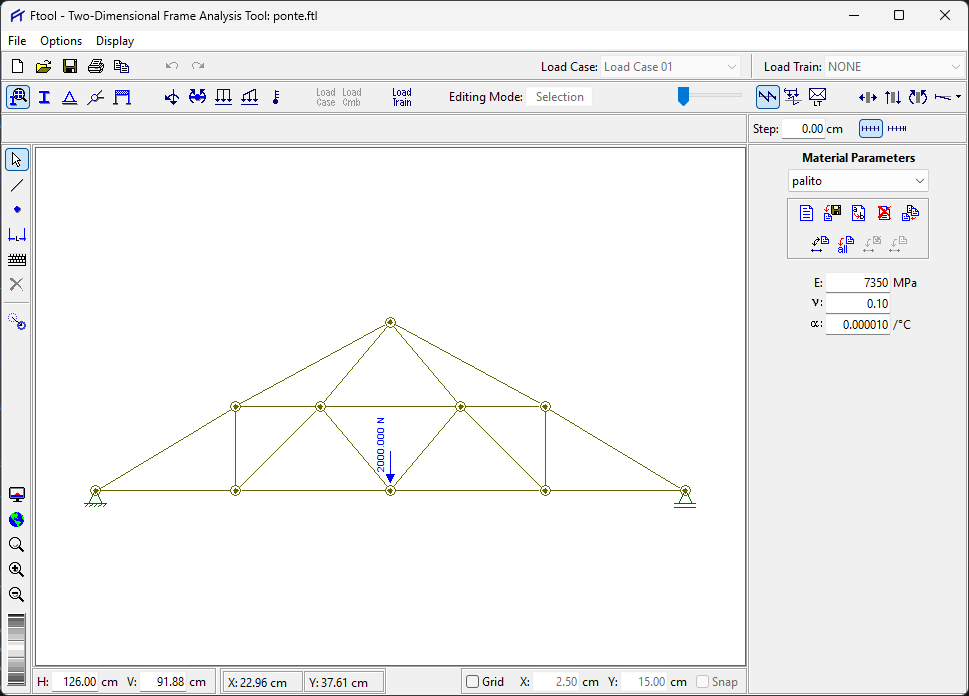
\includegraphics[width=.85\textwidth]{lib/figuras/ponte-ftool}
    \fonte{Elaborado pelo autor.}
\end{figure}

A Figura~\ref{fig:ponte-reconstruida} apresenta a geometria reconstruída pela ferramenta desenvolvida a partir da interpretação do arquivo \texttt{ponte.ftl}. Essa visualização corresponde ao modelo obtido computacionalmente após a leitura e a organização das informações estruturais contidas no arquivo.

\begin{figure}[H]
    \centering
    \caption{Geometria reconstruída pela ferramenta a partir do arquivo \texttt{ponte.ftl}.}
    \label{fig:ponte-reconstruida}
    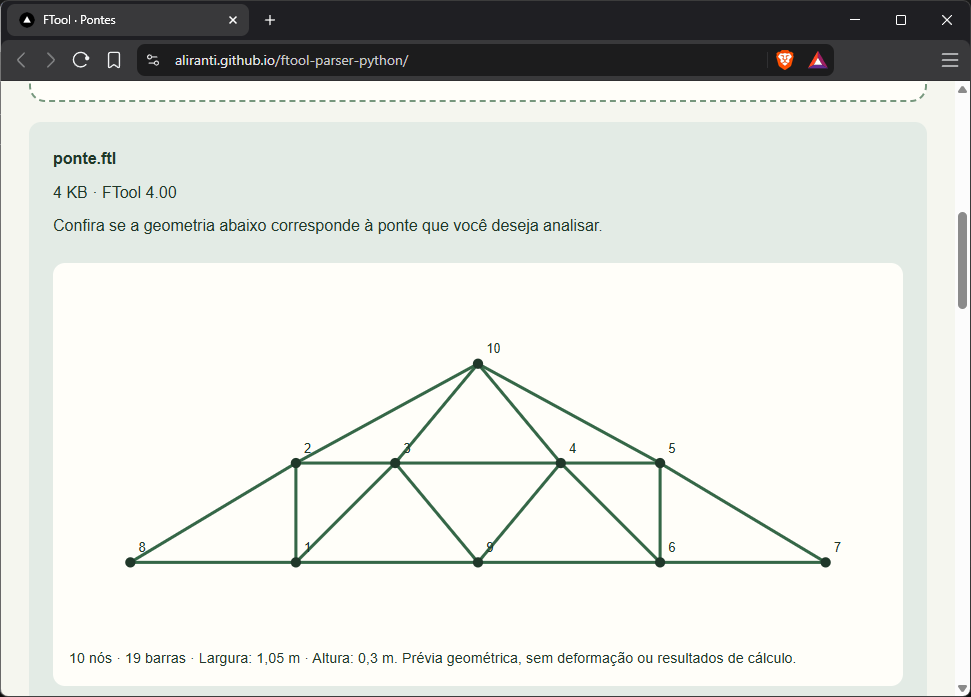
\includegraphics[width=.85\textwidth]{lib/figuras/ponte-reconstruida}
    \fonte{Elaborado pelo autor.}
\end{figure}

A comparação entre as Figuras~\ref{fig:ponte-ftool} e \ref{fig:ponte-reconstruida} indica correspondência entre a geometria original definida no FTOOL e o modelo reconstruído pela ferramenta. Essa equivalência é observada na configuração global da estrutura, na disposição dos elementos e na conectividade entre os nós e as barras, evidenciando que a interpretação do arquivo fornece uma representação compatível com o modelo estrutural de origem.

Além da reconstrução geométrica, foi verificada a equivalência entre diferentes formas de leitura do arquivo. O parser permite interpretar o modelo diretamente de um arquivo, de seu conteúdo textual ou de uma sequência de bytes. Os testes automatizados comparam as representações produzidas por essas três formas de entrada, verificando a consistência dos dados independentemente do procedimento de leitura.

Essa verificação é particularmente relevante para a aplicação web, uma vez que o arquivo FTL é processado diretamente na memória do navegador, sem a necessidade de armazenamento temporário no dispositivo.

Os resultados da interpretação são utilizados na etapa seguinte para a construção do modelo de análise estrutural. Dessa forma, a reconstrução da geometria, da conectividade e das propriedades dos elementos estabelece a base necessária para a determinação dos esforços internos, deslocamentos e reações de apoio, cujos resultados são apresentados na Seção~\ref{sec:resultados-analise}.

\section{Verificação da análise estrutural}
\label{sec:resultados-analise}

A verificação da análise estrutural foi realizada por meio da comparação entre os esforços axiais obtidos no FTOOL e aqueles calculados pela ferramenta desenvolvida, utilizando a biblioteca anaStruct. Para essa avaliação, foi empregado o modelo da ponte apresentado na seção anterior, composto por 10 nós e 19 barras.

O modelo analisado representa uma única face da ponte treliçada, submetida a um carregamento vertical de 2,00 kN (2000 N). Portanto, os esforços axiais, deslocamentos e reações de apoio obtidos correspondem exclusivamente à face representada no modelo, não devendo ser interpretados como resultados da estrutura tridimensional completa.

Para assegurar a comparabilidade, foram consideradas as mesmas condições de carregamento, apoio e propriedades estruturais nos dois ambientes de análise. A avaliação concentrou-se na correspondência entre os esforços axiais calculados, considerando tanto suas magnitudes quanto a identificação dos elementos tracionados e comprimidos.

A Figura~\ref{fig:axial-ftool} apresenta o diagrama de esforços axiais obtido no FTOOL.

\begin{figure}[H]
    \centering
    \caption{Diagrama de esforços normais da ponte no FTOOL.}
    \label{fig:axial-ftool}
    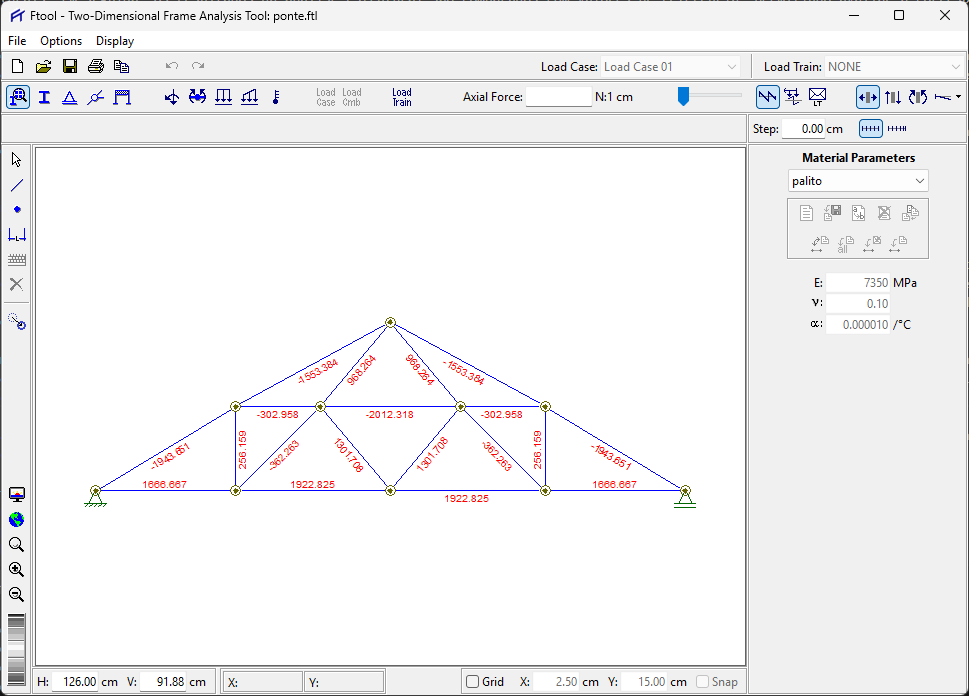
\includegraphics[width=0.85\textwidth]
        {lib/figuras/axial-ftool}
    \fonte{Elaborado pelo autor.}
\end{figure}

A Figura~\ref{fig:axial-ferramenta} apresenta o diagrama correspondente produzido pela ferramenta desenvolvida, a partir dos resultados da análise realizada com a biblioteca anaStruct.

\begin{figure}[H]
    \centering
    \caption{Diagrama de esforços normais produzido pela
    ferramenta desenvolvida.}
    \label{fig:axial-ferramenta}
    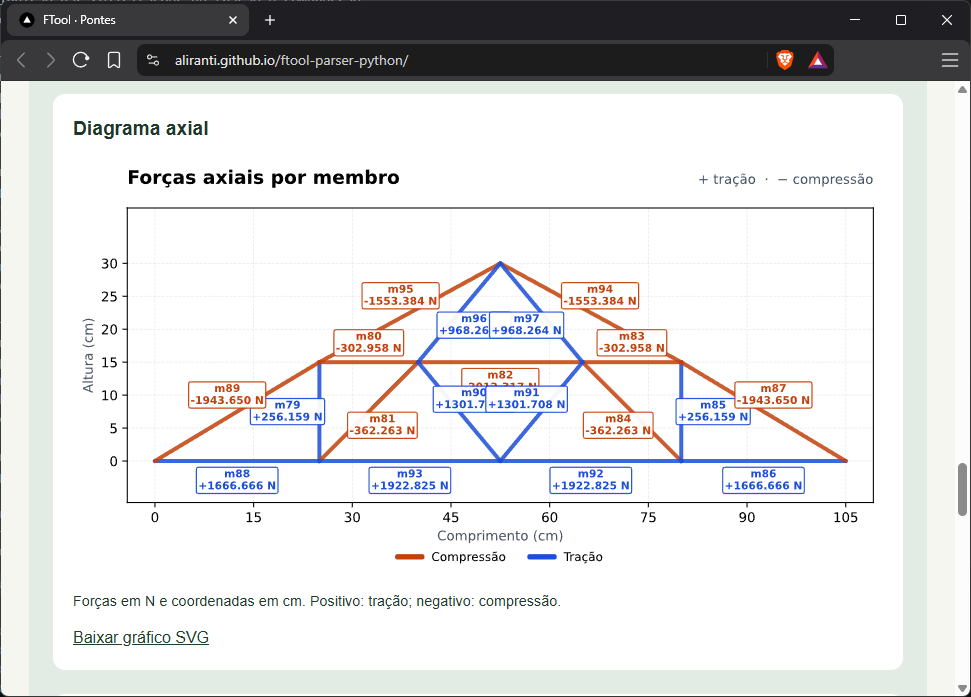
\includegraphics[width=0.85\textwidth]
        {lib/figuras/axial-ferramenta}
    \fonte{Elaborado pelo autor.}
\end{figure}

A comparação numérica foi realizada a partir dos esforços axiais apresentados pelos dois programas. Para cada barra, foi calculada a diferença absoluta entre o resultado obtido no FTOOL e aquele produzido pela ferramenta desenvolvida, conforme a Equação~\ref{eq:diferenca-esforco-axial}.

\begin{equation}
    \Delta N = \left|N_{\mathrm{FTOOL}} - N_{\mathrm{ferramenta}}\right|
    \label{eq:diferenca-esforco-axial}
\end{equation}

\noindent em que \(N_{\mathrm{FTOOL}}\) representa o esforço axial obtido no FTOOL e \(N_{\mathrm{ferramenta}}\) corresponde ao resultado fornecido pela ferramenta desenvolvida.

A Tabela~\ref{tab:comparacao-esforcos-axiais} apresenta os esforços axiais e suas diferenças absolutas para as 19 barras do modelo.

\begin{table}[H]
    \centering
    \caption{Comparação dos esforços axiais obtidos no FTOOL e na ferramenta desenvolvida.}
    \label{tab:comparacao-esforcos-axiais}
    \small
    \begin{tabular}{crrr}
        \hline
        \textbf{Barra} &
        \textbf{FTOOL (N)} &
        \textbf{Ferramenta (N)} &
        \textbf{$\Delta N$ (N)} \\
        \hline
        m79 &  256,159 &  256,159 & 0,000 \\
        m80 & -302,958 & -302,958 & 0,000 \\
        m81 & -362,263 & -362,263 & 0,000 \\
        m82 & -2012,318 & -2012,318 & 0,000 \\
        m83 & -302,958 & -302,958 & 0,000 \\
        m84 & -362,263 & -362,263 & 0,000 \\
        m85 &  256,159 &  256,159 & 0,000 \\
        m86 &  1666,667 &  1666,666 & 0,001 \\
        m87 & -1943,651 & -1943,650 & 0,001 \\
        m88 &  1666,667 &  1666,666 & 0,001 \\
        m89 & -1943,651 & -1943,650 & 0,001 \\
        m90 &  1301,708 &  1301,708 & 0,000 \\
        m91 &  1301,708 &  1301,708 & 0,000 \\
        m92 &  1922,825 &  1922,825 & 0,000 \\
        m93 &  1922,825 &  1922,825 & 0,000 \\
        m94 & -1553,384 & -1553,384 & 0,000 \\
        m95 & -1553,384 & -1553,384 & 0,000 \\
        m96 &  968,264 &  968,264 & 0,000 \\
        m97 &  968,264 &  968,264 & 0,000 \\
        \hline
    \end{tabular}
    \fonte{Elaborado pelo autor.}
\end{table}

Os resultados da Tabela~\ref{tab:comparacao-esforcos-axiais} demonstram correspondência entre os esforços axiais calculados pelo FTOOL e pela ferramenta desenvolvida, tanto em magnitude quanto na identificação dos elementos tracionados e comprimidos.

As diferenças absolutas calculadas a partir dos valores apresentados não ultrapassaram 0,001 N, sendo observadas nas barras m86, m87, m88 e m89. Nas demais barras, os resultados coincidiram até a terceira casa decimal. As pequenas diferenças são compatíveis com arredondamentos na apresentação dos valores, embora sua origem exata não tenha sido investigada.

Essa correspondência constitui uma evidência da consistência da interpretação do arquivo FTL e da conversão do modelo estrutural para a biblioteca anaStruct nas condições avaliadas. Ressalta-se que a comparação corresponde a uma única face da ponte submetida ao carregamento vertical de 2,00 kN. Portanto, os resultados não representam uma validação do comportamento tridimensional da ponte construída, nem permitem determinar sua carga de ruptura experimental.

\section{Resultados do pré-dimensionamento}
\label{sec:resultados-pre-dimensionamento}

Após a verificação dos resultados da análise estrutural, os esforços axiais obtidos para as barras do modelo \texttt{ponte.ftl} foram utilizados nas rotinas de pré-dimensionamento desenvolvidas neste trabalho. Essa etapa teve como objetivo estimar a quantidade de camadas necessária para cada elemento, considerando as solicitações de tração e compressão, os critérios de estabilidade e o padrão construtivo adotado.

As verificações foram realizadas com base nas propriedades geométricas e mecânicas configuradas na ferramenta. Para as barras tracionadas, foi considerada a resistência à tração paralela às fibras, enquanto as barras comprimidas foram avaliadas quanto à resistência e à estabilidade nos dois eixos principais da seção transversal.

A quantidade de camadas atribuída a cada barra corresponde à condição mais restritiva entre as verificações realizadas, respeitando o mínimo construtivo de três camadas definido na configuração padrão. Dessa forma, a composição das barras não depende exclusivamente da magnitude dos esforços axiais, mas também das condições de estabilidade e dos critérios construtivos estabelecidos.

A Figura~\ref{fig:resultado-camadas} apresenta a distribuição das quantidades de camadas obtidas para os elementos da estrutura, permitindo identificar as barras que exigem maior quantidade de material.

\begin{figure}[H]
    \centering
    \caption{Distribuição da quantidade de camadas
    obtida pelo pré-dimensionamento da ponte.}
    \label{fig:resultado-camadas}
    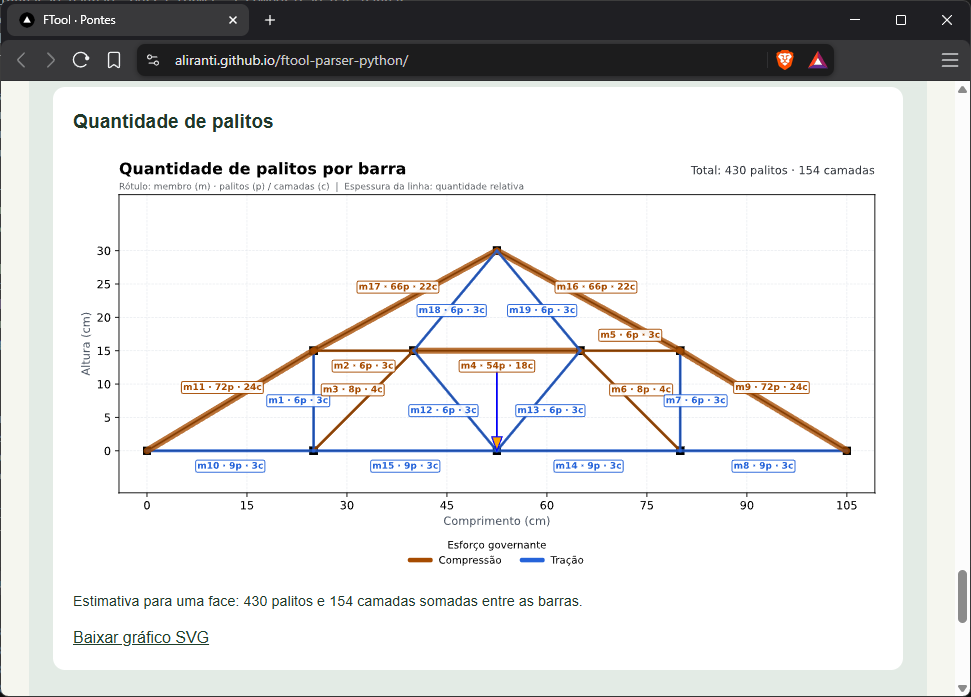
\includegraphics[width=0.85\textwidth]
        {lib/figuras/resultado-camadas}
    \fonte{Elaborado pelo autor.}
\end{figure}

Observa-se que as maiores quantidades de camadas foram atribuídas a determinados elementos comprimidos, com destaque para as barras m9 e m11, que apresentaram 24 camadas e 72 palitos cada. A barra m4 também apresentou uma quantidade expressiva, com 18 camadas e 54 palitos.

Em contrapartida, as barras tracionadas apresentaram, predominantemente, três camadas, correspondentes ao mínimo construtivo adotado. Essa diferença evidencia a influência das verificações de estabilidade no pré-dimensionamento dos elementos comprimidos, uma vez que sua resistência não depende exclusivamente da área da seção transversal, mas também das condições de esbeltez e flambagem.

Para o modelo analisado, a estimativa total correspondeu a 430 palitos distribuídos entre as 19 barras, com uma soma de 154 camadas. Esses resultados demonstram a distribuição não uniforme do material entre os elementos da estrutura, determinada pelas solicitações axiais e pelos critérios resistentes e construtivos estabelecidos.

Além da definição das seções compostas, a ferramenta realiza a estimativa da quantidade física de palitos necessária para a construção das barras. Para isso, são considerados os comprimentos dos elementos, o número de camadas e o comprimento comercial dos palitos, conforme o procedimento descrito na metodologia.

Os resultados de referência do processamento são apresentados na Tabela~\ref{tab:resultado-palitos}.

\begin{table}[H]
    \centering
    \caption{Resumo dos resultados do pré-dimensionamento
    do modelo analisado.}
    \label{tab:resultado-palitos}
    \begin{tabular}{lr}
        \hline
        \textbf{Grandeza} & \textbf{Valor} \\
        \hline
        Quantidade de barras & 19 \\
        Soma das camadas das barras & 154 \\
        Quantidade estimada de palitos no modelo & 430 \\
        Estimativa para duas faces idênticas & 860 \\
        Mínimo construtivo por barra & 3 \\
        Comprimento comercial do palito (mm) & 115 \\
        Sobreposição padrão nas emendas (mm) & 0 \\
        \hline
    \end{tabular}
    \fonte{Elaborado pelo autor.}
\end{table}

Os valores apresentados distinguem a quantidade de camadas necessária à composição das seções transversais da quantidade física de palitos estimada para a construção dos elementos. A soma das camadas corresponde ao total das quantidades atribuídas individualmente às barras, não representando, portanto, a quantidade de palitos comerciais utilizados.

Para o modelo analisado, a estimativa registrada nos testes de referência corresponde a 430 palitos. Considerando duas faces estruturais idênticas, esse valor é duplicado, resultando em uma estimativa de 860 palitos. Essa quantidade não inclui elementos adicionais de ligação transversal, travamento ou eventuais perdas de material durante a fabricação.

Cabe destacar que os resultados constituem estimativas de pré-dimensionamento, obtidas a partir das propriedades adotadas e das hipóteses de cálculo implementadas. Assim, a quantidade estimada de palitos não corresponde necessariamente à quantidade empregada na construção física da ponte.

A comparação entre esses resultados e as estimativas obtidas por meio da planilha eletrônica preexistente é apresentada na Seção~\ref{sec:resultados-comparacao}.

\section{Aplicação web e integração dos módulos}
\label{sec:resultados-aplicacao-web}

A integração das rotinas de interpretação, análise estrutural e pré-dimensionamento resultou em uma aplicação web que permite executar as principais funcionalidades da ferramenta diretamente pelo navegador. A interface reúne as etapas de processamento em um único ambiente, desde a importação do modelo estrutural até a apresentação dos resultados.

A Figura~\ref{fig:web-interface-inicial} apresenta a página inicial da aplicação, na qual são disponibilizados o campo de importação dos arquivos FTL e uma descrição das principais etapas do processamento. A organização da interface busca orientar o usuário ao longo do procedimento, compreendendo a importação da estrutura, a análise dos esforços e o pré-dimensionamento das barras.

\begin{figure}[H]
    \centering
    \caption{Interface inicial da aplicação web desenvolvida.}
    \label{fig:web-interface-inicial}
    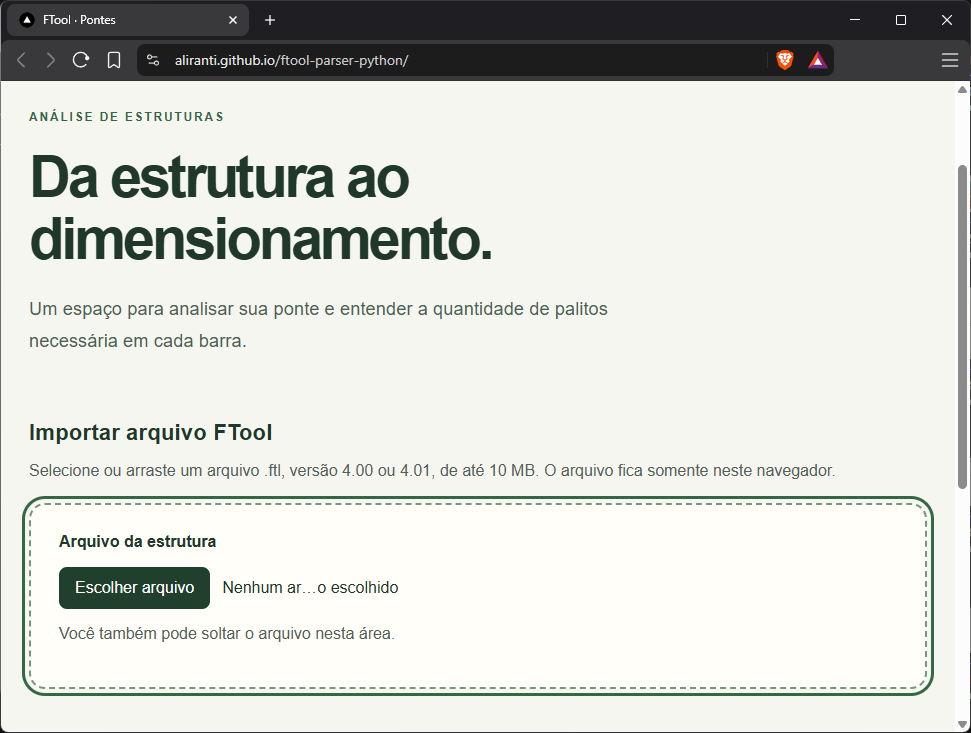
\includegraphics[width=0.95\textwidth]
        {lib/figuras/web-interface-inicial}
    \fonte{Elaborado pelo autor.}
\end{figure}

Após a seleção do arquivo, a ferramenta realiza sua interpretação e apresenta uma visualização preliminar da geometria estrutural, conforme demonstrado anteriormente na Figura~\ref{fig:ponte-reconstruida}. Essa etapa permite conferir o modelo antes da execução dos cálculos.

Além da visualização inicial, a aplicação disponibiliza uma interface para configuração dos parâmetros utilizados na análise estrutural e no pré-dimensionamento. O usuário pode consultar e modificar propriedades dos materiais, características geométricas das seções e critérios empregados nas verificações de resistência e estabilidade. As alterações são aplicadas somente ao processamento corrente, sem modificar o arquivo FTL original.

Após a confirmação do modelo e dos parâmetros selecionados, a aplicação executa as rotinas de análise estrutural e pré-dimensionamento. Os resultados são apresentados por meio de diagramas de esforços axiais, representação da configuração deformada e distribuição da quantidade estimada de palitos, além de informações numéricas relativas às barras e às reações de apoio.

Para reunir essas informações, foi desenvolvida uma interface de relatório consolidado. A Figura~\ref{fig:web-relatorio} apresenta parte desse relatório, contendo indicadores-resumo e uma tabela com os resultados do processamento para cada barra da estrutura.

\begin{figure}[H]
    \centering
    \caption{Relatório consolidado dos resultados
    gerados pela aplicação web.}
    \label{fig:web-relatorio}
    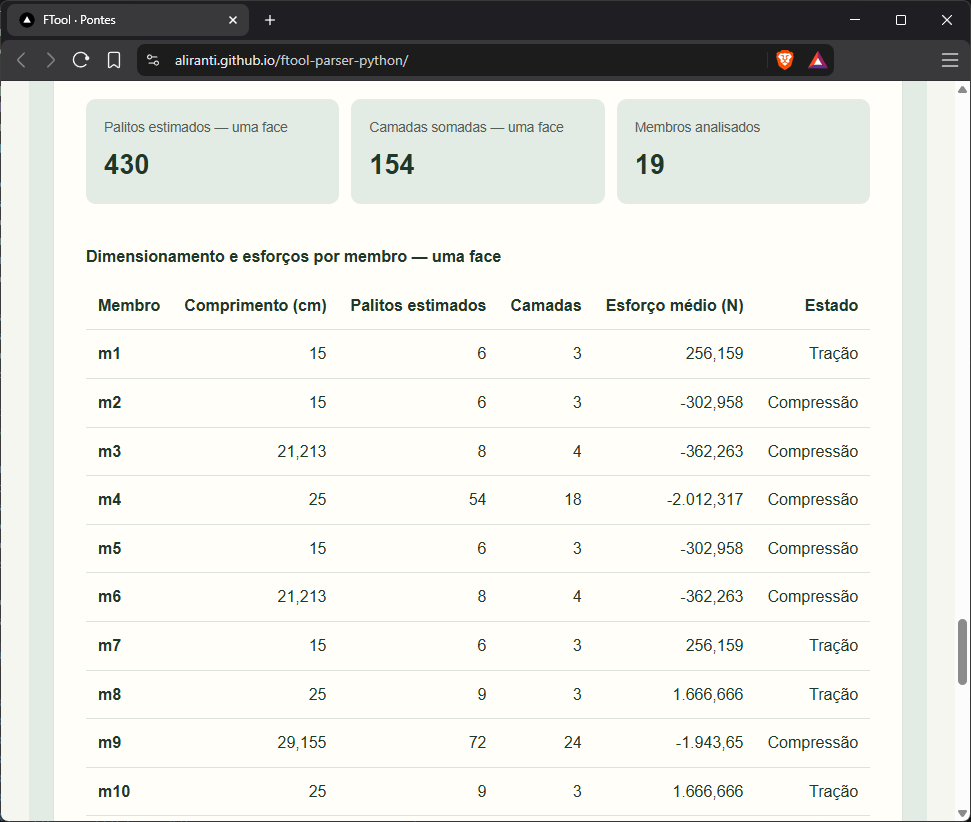
\includegraphics[width=0.95\textwidth]
        {lib/figuras/web-relatorio}
    \fonte{Elaborado pelo autor.}
\end{figure}

O relatório reúne os resultados da análise e do pré-dimensionamento. Os indicadores mostram os totais de palitos, camadas e barras. A tabela detalha, por barra, o comprimento, as quantidades de palitos e camadas, o esforço axial e o tipo de solicitação.

Para o modelo \texttt{ponte.ftl}, o relatório apresentou uma estimativa de 430 palitos, 154 camadas somadas entre as barras e 19 elementos analisados, considerando uma face da estrutura. Esses valores correspondem aos resultados de pré-dimensionamento discutidos na Seção~\ref{sec:resultados-pre-dimensionamento}.

A comunicação entre a interface web e as rotinas Python é realizada por meio do Pyodide, com o processamento executado em um Web Worker. Os resultados são transferidos entre os módulos por meio de estruturas serializadas em JSON, permitindo sua utilização pelos componentes responsáveis pela apresentação gráfica e numérica.

A implementação demonstra a integração das diferentes etapas computacionais em uma única aplicação, permitindo ao usuário importar modelos estruturais, configurar parâmetros e consultar os resultados sem a necessidade de executar diretamente as rotinas Python. Dessa forma, a ferramenta disponibiliza as funcionalidades desenvolvidas em uma interface destinada à análise e ao pré-dimensionamento de pontes treliçadas de palitos de picolé.

\section{Comparação entre o dimensionamento original e a ferramenta desenvolvida}
\label{sec:resultados-comparacao}

Conforme descrito na Seção~\ref{sec:metodologia-comparacao-planilha}, foi realizada uma comparação entre um procedimento de pré-dimensionamento baseado em planilha eletrônica e aquele implementado na ferramenta desenvolvida. A planilha foi utilizada anteriormente ao desenvolvimento do software, durante o planejamento de uma ponte de palitos de picolé posteriormente construída e submetida a ensaio experimental.

Para a comparação, foi utilizada uma cópia da planilha, preenchida com os comprimentos e esforços axiais das 19 barras do modelo estrutural analisado neste trabalho. Esse modelo corresponde a uma única face da ponte, submetida a um carregamento vertical de 2,00 kN. Desse modo, os dados empregados na comparação representam as solicitações de uma face isolada, e não o comportamento global da estrutura física.

A Figura~\ref{fig:planilha-comparacao} apresenta a planilha preenchida com os dados do modelo. Observa-se que o procedimento utiliza informações relativas ao comprimento e ao esforço axial das barras, além de etapas intermediárias denominadas Análise 1 e Análise 2, empregadas na estimativa da quantidade de camadas e de palitos.

\begin{figure}[H]
    \centering
    \caption{Planilha de pré-dimensionamento preenchida
    com os dados das barras da face analisada.}
    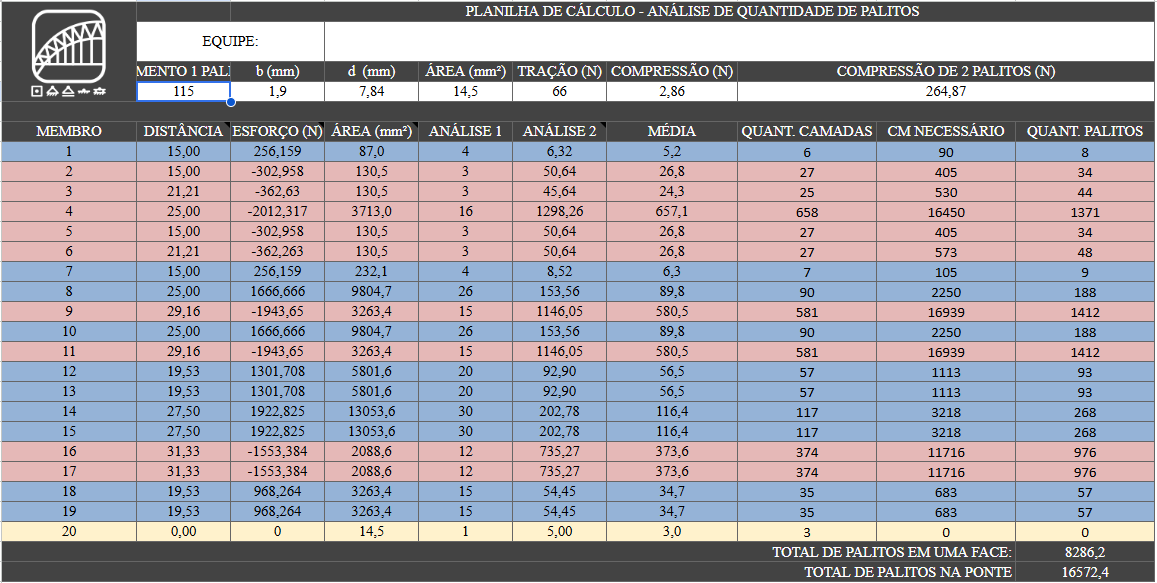
\includegraphics[width=0.95\textwidth]
        {lib/figuras/planilha-comparacao}
    \label{fig:planilha-comparacao}
    \fonte{Elaborado pelo autor a partir da planilha preexistente.}
\end{figure}

A análise das fórmulas da planilha permitiu identificar diferenças em relação ao procedimento implementado na ferramenta. Na primeira etapa, denominada Análise 1, é determinada uma quantidade inicial de elementos, a partir do esforço axial solicitante e de parâmetros de resistência previamente estabelecidos.

Posteriormente, o resultado da primeira análise é utilizado no cálculo de uma área transversal, conforme a Equação~\ref{eq:area-planilha}.

\begin{equation}
    A_p = (n_1 b)(n_1 d) = n_1^2 bd
    \label{eq:area-planilha}
\end{equation}

\noindent em que $A_p$ representa a área calculada pela planilha, $n_1$ corresponde ao resultado da primeira análise e $b$ e $d$ são as dimensões transversais adotadas para o palito.

Nessa expressão, as duas dimensões transversais são multiplicadas por $n_1$, fazendo com que a área calculada seja proporcional ao quadrado dessa quantidade. Esse procedimento difere da composição geométrica adotada pela ferramenta desenvolvida, na qual a adição de camadas ocorre pela espessura do palito, produzindo uma área proporcional ao número de camadas.

Na segunda etapa, para as barras comprimidas, a planilha utiliza a área obtida anteriormente e um parâmetro numérico de valor 2,86, conforme a Equação~\ref{eq:analise2-planilha}.

\begin{equation}
    n_2 = \frac{A_p}{2,86}
    \label{eq:analise2-planilha}
\end{equation}

Em determinadas barras, a fórmula inclui ainda um acréscimo fixo de cinco unidades. Os resultados das duas análises são combinados por uma média aritmética, com arredondamento para cima nos casos examinados, conforme a Equação~\ref{eq:camadas-planilha}.

\begin{equation}
    n_p =
    \left\lceil
    \frac{n_1+n_2}{2}
    \right\rceil
    \label{eq:camadas-planilha}
\end{equation}

\noindent em que $n_p$ representa a quantidade final de camadas estimada pela planilha e $n_2$ corresponde ao resultado da segunda análise, incluindo eventuais acréscimos estabelecidos na célula.

A Tabela~\ref{tab:comparacao-camadas} apresenta os resultados de três barras comprimidas, selecionadas por apresentarem diferenças expressivas entre as estimativas dos dois procedimentos. Nesta comparação, a planilha e o relatório de pré-dimensionamento empregam a identificação sequencial de m1 a m19, enquanto a tabela de esforços axiais apresentada na Seção~\ref{sec:resultados-analise} conserva os identificadores originais dos elementos no FTOOL (m79 a m97).

\begin{table}[H]
    \centering
    \caption{Comparação da quantidade de camadas
    estimada para barras comprimidas.}
    \label{tab:comparacao-camadas}
    \begin{tabular}{c c c c}
        \hline
        \textbf{Barra} &
        \textbf{Esforço (N)} &
        \textbf{Planilha} &
        \textbf{Ferramenta} \\
        \hline
        m4  & $-2012,318$ & 658 & 18 \\
        m9  & $-1943,651$ & 581 & 24 \\
        m11 & $-1943,651$ & 581 & 24 \\
        \hline
    \end{tabular}
    \fonte{Elaborado pelo autor.}
\end{table}

Para exemplificar o cálculo da planilha, considera-se a barra m4, submetida a um esforço axial de compressão de aproximadamente 2012,318 N. A primeira análise resultou em 16 unidades. Considerando as dimensões de 1,85 mm e 7,84 mm, a área calculada foi de 3713,024 mm$^2$, conforme a Equação~\ref{eq:exemplo-area-planilha}.

\begin{equation}
    A_p =
    (16 \cdot 1,85)(16 \cdot 7,84)
    = 3713,024\ \mathrm{mm}^2
    \label{eq:exemplo-area-planilha}
\end{equation}

Na sequência, a segunda análise produziu um resultado de aproximadamente 1298,26. A quantidade final de camadas foi então calculada por

\begin{equation}
    n_p =
    \left\lceil
    \frac{16+1298,26}{2}
    \right\rceil
    = 658.
    \label{eq:exemplo-camadas-planilha}
\end{equation}

Para a mesma barra, a ferramenta desenvolvida estimou 18 camadas. Essa diferença está associada às formulações empregadas pelos procedimentos. Enquanto a planilha combina estimativas intermediárias, a ferramenta realiza verificações iterativas de resistência e estabilidade, considerando a geometria da seção composta, os esforços solicitantes e os critérios de esbeltez adotados.

As diferenças também se manifestam na estimativa da quantidade total de palitos. Na cópia examinada, embora o parâmetro nominal de comprimento comercial tenha sido atualizado para 115 mm, as fórmulas de contabilização dos palitos ainda dividem o comprimento acumulado das camadas pelo valor fixo de 12 cm. Posteriormente, é acrescentada uma margem de 10\%. Portanto, os totais apresentados pela planilha refletem esse divisor ainda não atualizado, e não uma contagem integralmente padronizada para 115 mm. Para uma face da ponte, o procedimento é representado pela Equação~\ref{eq:total-planilha}.

\begin{equation}
    P_p =
    1,10
    \left(
        \frac{\displaystyle\sum_{i=1}^{19}L_i n_{p,i}}
        {12}
    \right)
    \label{eq:total-planilha}
\end{equation}

\noindent em que $P_p$ representa a estimativa total de palitos para uma face, $L_i$ corresponde ao comprimento da barra $i$, em centímetros, e $n_{p,i}$ representa a quantidade de camadas atribuída ao elemento pela planilha.

A ferramenta desenvolvida, por sua vez, estima a quantidade inteira de palitos necessários em cada barra, considerando seu comprimento, o número de camadas e a configuração adotada para as emendas. Na configuração padrão utilizada nesta avaliação, o comprimento comercial corresponde a 115 mm, com sobreposição nula nas emendas. Embora o campo de comprimento da planilha também indique 115 mm, as fórmulas responsáveis pelos totais ainda utilizam 12 cm; a comparação dos valores globais preserva os resultados efetivamente calculados nessa versão da planilha.

A Tabela~\ref{tab:comparacao-totais} sintetiza os resultados globais apresentados pelos dois procedimentos.

\begin{table}[H]
    \centering
    \caption{Comparação das estimativas de palitos
    para o modelo analisado.}
    \label{tab:comparacao-totais}
    \begin{tabular}{p{6cm}r r}
        \hline
        \textbf{Grandeza} &
        \textbf{Planilha} &
        \textbf{Ferramenta} \\
        \hline
        Barras analisadas & 19 & 19 \\
        Palitos estimados para uma face
            & 8286,21 & 430 \\
        Palitos estimados para duas faces
            & 16572,43 & 860 \\
        \hline
    \end{tabular}
    \fonte{Elaborado pelo autor.}
\end{table}

Os valores apresentados demonstram diferenças expressivas entre as estimativas. Entretanto, essas quantidades não representam uma comparação sob condições integralmente equivalentes: além das diferenças nos critérios de dimensionamento, nas propriedades geométricas e resistentes e nas regras de contabilização do material, o divisor usado nas fórmulas de totalização da planilha ainda corresponde a 12 cm. Assim, a diferença entre os totais não pode ser atribuída exclusivamente à formulação da área da seção transversal.

Além disso, os valores fracionários obtidos pela planilha representam uma estimativa contínua do comprimento total de palitos, enquanto os valores da ferramenta correspondem à soma de quantidades inteiras estimadas para cada barra. Dessa forma, a diferença entre os totais não deve ser interpretada isoladamente como medida de precisão ou de eficiência estrutural.

As estimativas apresentadas para duas faces correspondem à duplicação dos resultados obtidos para a face analisada. Essa aproximação pressupõe duas faces com composição equivalente e não contempla, necessariamente, os elementos adicionais de ligação e travamento transversal presentes em uma ponte tridimensional.

Outro aspecto identificado na planilha está relacionado à interpretação dimensional das fórmulas, especialmente na divisão de uma grandeza de área por um parâmetro identificado como resistência em força. Sem a definição de uma relação física compatível entre essas grandezas, os resultados não podem ser considerados diretamente equivalentes às verificações resistentes implementadas na ferramenta desenvolvida.

A ponte associada ao procedimento original foi construída anteriormente ao desenvolvimento do software e submetida a um ensaio experimental de carregamento até a ruptura. Nesse ensaio, a estrutura completa atingiu uma carga correspondente a uma massa de 246 kg, equivalente a aproximadamente 2,41 kN, considerando uma aceleração gravitacional de 9,81 m/s$^2$.

É importante distinguir esse resultado experimental do carregamento utilizado na avaliação numérica. O modelo analisado neste trabalho representa apenas uma das faces da ponte, submetida a uma força vertical de 2,00 kN, enquanto o carregamento experimental foi aplicado à estrutura física completa, composta por duas faces e elementos de ligação transversal.

Assim, os valores de carregamento não são diretamente comparáveis sem considerar a distribuição das forças entre as faces, as condições reais de ligação e o comportamento global da estrutura. Além disso, o software desenvolvido realiza verificações de pré-dimensionamento, não uma simulação completa do processo de ruptura.

O resultado do ensaio é, portanto, utilizado como informação experimental complementar sobre a ponte construída, não constituindo uma validação da previsão de ruptura da ferramenta desenvolvida.

A comparação evidencia as diferenças entre o procedimento anteriormente empregado e a abordagem implementada neste trabalho. A principal contribuição da ferramenta desenvolvida consiste na integração da interpretação geométrica, da análise estrutural e do pré-dimensionamento, com parâmetros configuráveis e resultados individualizados por barra, reduzindo a necessidade de transferência manual de informações entre as etapas.

\section{Limitações da ferramenta desenvolvida}
\label{sec:resultados-limitacoes}

Embora os resultados apresentados nas seções anteriores demonstrem a integração das etapas de interpretação, análise estrutural e pré-dimensionamento, a ferramenta desenvolvida apresenta limitações relacionadas às hipóteses de modelagem, às propriedades dos materiais e à representação do comportamento físico das pontes construídas com palitos de picolé.

A primeira limitação está relacionada à representação estrutural bidimensional. Os modelos utilizados na análise correspondem a uma face da ponte, não sendo considerados diretamente os efeitos decorrentes do comportamento tridimensional da estrutura completa. Dessa forma, a contribuição dos elementos de ligação transversal, a distribuição efetiva dos carregamentos entre as faces e possíveis instabilidades fora do plano não são avaliadas integralmente.

Outra limitação está associada às propriedades mecânicas dos palitos. Os parâmetros utilizados nas verificações de resistência e estabilidade correspondem a valores adotados para o cálculo, não tendo sido determinados por meio de ensaios experimentais específicos com os materiais empregados na construção da ponte. Consequentemente, variações naturais da madeira, defeitos dos palitos e diferenças entre lotes podem produzir comportamentos distintos daqueles previstos pelo modelo.

No pré-dimensionamento, as camadas de palitos são consideradas integralmente solidárias, formando uma seção transversal equivalente. Essa hipótese desconsidera possíveis deslocamentos relativos entre os elementos, imperfeições de colagem e alterações na rigidez decorrentes das emendas. A influência da resistência do adesivo e dos mecanismos de falha das ligações também não é avaliada diretamente pelas rotinas implementadas.

A estimativa da quantidade de palitos constitui outra simplificação. O cálculo considera o comprimento das barras, a quantidade de camadas e a sobreposição configurada para as emendas, mas não contempla automaticamente perdas de material durante o corte e a montagem, palitos descartados por defeitos ou elementos adicionais necessários à construção da estrutura completa. Assim, os quantitativos apresentados representam estimativas de material para as barras analisadas, e não uma lista definitiva de consumo na fabricação.

Também existem limitações relacionadas ao pré-dimensionamento dos elementos comprimidos. As verificações de estabilidade são realizadas a partir de propriedades geométricas equivalentes e parâmetros normativos adotados como referência. Entretanto, a aplicação desses critérios a elementos compostos por palitos colados envolve hipóteses simplificadoras, especialmente quanto à rigidez das ligações e ao comportamento conjunto das camadas.

Quanto à interpretação dos arquivos FTL, a implementação foi desenvolvida e verificada para as versões e os componentes estruturais contemplados nos testes realizados. Desse modo, não é possível assegurar a compatibilidade com todas as funcionalidades do FTOOL ou com eventuais alterações futuras no formato de armazenamento dos arquivos.

Por fim, as verificações realizadas neste trabalho concentram-se na consistência da interpretação, na correspondência dos resultados de análise estrutural e no comportamento das rotinas de pré-dimensionamento diante dos critérios implementados. Embora tenha sido apresentado um resultado experimental de uma ponte previamente construída, não foi realizada uma campanha de ensaios destinada à validação das estimativas de resistência ou à previsão da carga de ruptura das estruturas.

Dessa forma, a ferramenta deve ser compreendida como um recurso de apoio à análise estrutural e ao pré-dimensionamento de pontes treliçadas de palitos de picolé. Seus resultados fornecem estimativas baseadas nas hipóteses e nos parâmetros adotados, não substituindo a avaliação experimental das propriedades dos materiais e do comportamento das estruturas construídas.
